\documentclass[a4paper]{article}

\usepackage{amsthm}

\usepackage{tikz}

\newtheorem{lemma}{Lemma}
\newtheorem{proposition}{Proposition}


\title{Coloring de Bruijn graphs}

\author{Johannes Marti and Leif Sabellek}

\begin{document}

\maketitle

\section*{Notation}

If a length $k$ is obvious from the context we write $w\dots$ for $w \in
\{0,1\}^+$ for the word $w w w w w w w w w w w w \dots$ truncated at
length $k$. Usually the length of $w$ will be smaller than $k$.

We assume that the pattern is such that every node has either just
outgoing $0$-edges or just outgoing $1$-edges. Then call a node a
$i$-node if it has just outgoing $i$-edges. A coloring for $n$-$m$ colors
is then a coloring with a pattern that has at most $n$ many $0$-nodes
and at most $m$ many $1$-nodes.

\section*{$2$-$2$ colors}

The following is a $2$-$2$ pattern that colors $T_3$ but not $T_2$:
\begin{center}
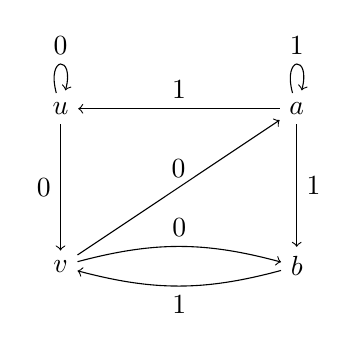
\begin{tikzpicture}
 \node (u) at (0,2) {$u$};
 \node (v) at (0,0)  {$v$};

 \node (a) at (3,2) {$a$};
 \node (b) at (3,0)  {$b$};

 \draw [->] (u) edge node[left] {$0$} (v);
 \draw [->] (u) edge [loop above] node[above] {$0$} (u);

 \draw [->] (a) edge node[right] {$1$} (b);
 \draw [->] (a) edge [loop above] node[above] {$1$} (a);

 \draw [->] (v) edge node[above] {$0$} (a);
 \draw [->] (v) edge [bend left=15] node[above] {$0$} (b);

 \draw [->] (a) edge node[above] {$1$} (u);
 \draw [->] (b) edge [bend left=15] node[below] {$1$} (v);
\end{tikzpicture}
\end{center}

Our goal is to show that $T_3$ colors all colorable $2$-$2$ patterns. We
start with two lemmas.

\begin{lemma} \label{reachability lemma}
 If there is a homomorphism $h$ from $T_k$ to a $2$-$2$ pattern $P$ then
$h(0\dots) \rightarrow_0 s$ for all $0$-node $s$ in the image of $h$.
\end{lemma}
\begin{proof}
 First observe that $h(0\dots) \rightarrow_0 h(0\dots)$, because $h$ is
a homomorphism. Note that there is at most one $0$-node $s$ that is
distinct from $h(0\dots)$ because there are at most two $0$-nodes in
$P$. Assume that $s \neq h(0\dots)$ is in the image of $h$, that is, $s
= h(x)$ for some $x$ in $T_k$. We show that then $h(0\dots)
\rightarrow_0 s$. Because there is a $0$-path from $0\dots$ to $x$ in
$T_k$ there must also be a $0$-path from $h(0\dots)$ to $s$. All nodes
on this path are $0$-nodes and thus they are either equal to $h(0\dots)$
or to $s$ since $P$ does contain no more than two $0$-nodes. Consider
the first occurrence of $s$ on this path. It is not possible that this is
the start node of the path because $h(0\dots) \neq s$. But then the
predecessor of the first occurrence of $s$ must be $h(0\dots)$ and hence
$h(0\dots) \rightarrow_0 s$.
\end{proof}

\begin{lemma} \label{between lemma}
 If there is a homomorphism $h$ from $T_k$ to a $2$-$2$ pattern $P$ then
there is a $0$-node $s$ in $P$ such that $h(10\dots) \rightarrow_1
s \rightarrow_0 h(1\dots)$.
\end{lemma}
\begin{proof}
Consider a path $v_0 \rightarrow_1 v_1 \rightarrow_0
v_2 \rightarrow_1 \dots \rightarrow_0 v_l$ in $p$ from $v_0 =
h(10\dots)$ to $v_l = h(1\dots)$. This path must exists because it is
easy to see that an alternating $0$ and $1$ path from $10\dots$ to
$1\dots$ exists in $T_k$. note that $l$ is even because the path is
alternating. In fact one could argue more carefully that its length must
be largest even number smaller or equal to $k$.

We can proof the claim with in induction on the length of this path. If
the length of the path is $0$ then $h(10\dots) = h(1\dots)$ and thus we
can set $s = h(01\dots)$ because $h(10\dots) \rightarrow_1 h(01\dots)$
and $h(01\dots) \rightarrow_0 h(10\dots)$.

If the length $l$ of the path is larger than $0$ then it can be split
into a path $v_0 \rightarrow_1 \dots \rightarrow_0 v_{l - 2}$ and a
length $2$ path $v_{l - 2} \rightarrow_1 v_{l - 1} \rightarrow_0 v_l$.
Because $P$ contains at most two $1$-edges we have either that
$h(10\dots) = h(1\dots)$, or that $v_{l - 2} = h(10\dots)$, or that
$v_{l - 2} = h(1\dots)$.

In the first case where $h(10\dots) = h(1\dots)$ we have already seen that we
can set $s = h(01\dots)$.

In the case where $v_{l - 2} = h(10\dots)$ we can set $s = v_{l - 1}$
because $v_{l - 2} \rightarrow_1 v_{l - 1} \rightarrow_0 v_l$ and $v_l =
h(1,\dots)$.

In the last case where $v_{l - 2} = h(1\dots)$, we can simply apply the
induction hypothesis to the path $v_0 \rightarrow_1 \dots \rightarrow_0
v_{l - 2}$.
\end{proof}

\begin{proposition}[$T_3$ suffices for $2$-$2$ colors]
 Let $P$ be a $2$-$2$ pattern such that there is a homomorphism $h$ from
$T_k$, for some $k > 3$, to $P$. Then there is a homomorphism $g$ from
$T_3$ to $P$.
\end{proposition}
\begin{proof}
Define $g$ from $T_3$ to $P$ such that it maps as follows
\[
 \begin{array}{rcl}
 000 & \mapsto & h(0\dots) \\
 001 & \mapsto & h(0\dots) \\
 010 & \mapsto & h(01\dots) \\
 011 & \mapsto & s_0
 \end{array} \quad
 \begin{array}{rcl}
 111 & \mapsto & h(1\dots) \\
 110 & \mapsto & h(1\dots) \\
 101 & \mapsto & h(10\dots) \\
 100 & \mapsto & s_1
 \end{array}
\]
Here, $s_0$ is the node which exists by Lemma~\ref{between lemma} and
$s_1$ is the analogous node which exists by swapping all $0$s and $1$s
in the lemma. It is left to the reader to check that this defines a
homomorphism. At most edges this follows because $h$ is a homomorphism,
and for the more difficult edges one uses Lemmas \ref{reachability
lemma}~and~\ref{between lemma}.
\end{proof}
\end{document}
